% !TEX root = ../algo-summary.tex
\section{Dynamic Programming}\label{sec:dynamic_programming}


\textcolor{AccentBlue}{Greedy}. 
Build up a solution incrementally, myopically optimizing some local criterion.

\textcolor{AccentBlue}{Divide-and-conquer}. 
Break up a problem into two sub-problems of roughly equal size; 
solve each sub-problem independently; 
combine the two sub-problem solutions to form solution to original problem.

\textcolor{AccentRed}{Dynamic programming}. 
Break up a problem into many overlapping sub-problems; 
combine solutions to small subproblems to build up solutions to larger and larger sub-problems.
\begin{itemize}
\item overlapping sub-problem = a sub-problem whose results can be reused many times
\item Hint: express your optimal solution by a recursive formula
\end{itemize}
\medskip


Powerful technique for solving optimization problems, which have certain well-defined clean structural properties.
\begin{definition}[Principle of optimality]\label{def:principle_of_optimality}
\hl[5]{For the global problem to be solved optimally, each subproblem must be solved optimally.}
\end{definition}
this principle must hold to apply DP

The global optimal solution consists of optimal solutions to subproblems.

\medskip
Polynomial time DP:
\begin{itemize}
\item Polynomially-many distinct overlapping subproblems (polynomial in input size).
\item DP does not necessarily lead to a polynomial time algorithm
\end{itemize}
\medskip

DP selection principle: \hl{When given a set of feasible options to choose from, try them all and take the best}

\subsection{Weighted Interval Scheduling}
We denote by \(p(j)\) the largest index \(i\) with \(i < j\) and such that job \(i\) is compatible with \(j\), i.e.
\begin{equation}\label{eq:interval_scheduling_pj}
  p(j)
  :=
  \begin{cases}
    \max\{ i \mid f_i \leq s_j\} & \exists i \text{ with } f_i \leq s_j\\
    0 & \text{otherwise}
  \end{cases}
\end{equation}



\begin{algorithm}[h]
\caption{Compute \(p(j)\) values}\label{alg:compute_pj}
\begin{algorithmic}[1]
\Require Jobs \(1, \ldots, n\) sorted according to their finish time \(f_1 \leq \cdots \leq f_n\)
\State Sort all starting and finish times in a single array \(A\)
\State \(\texttt{index} \gets 0\)
\ForAll{\(e \in A\)} \Comment{go through all times (`events') in ascending order}
  \If{\(e = f_i\)}
    \State \(\texttt{index} \gets i\)
  \ElsIf{\(e = s_j\)}
    \State \(p[j] \gets \texttt{index}\)
  \EndIf
\EndFor
\end{algorithmic}
\end{algorithm}

The algorithm goes through every time slot, and it remembers the index of the last finish time.
When we encounter a starting time $s_j$, its $p$ value is the largest index $i$ such that $f_i \leq s_j$, which is exactly the value of \texttt{index} in the algorithm. 
Hence, \autoref{alg:compute_pj} is correct.

Sorting takes $O(n \log n)$ time, and it is easy to see that the for loop takes $O(n)$ time.



% \textcolor{AccentBlue}{Dynamic programming formulation.}
Assume jobs are labeled so that \(f_1 \le \cdots \le f_n\).
Let \(v_j\) be the value/weight of job \(j\), and let
\(
\operatorname{OPT}(j)
\)
denote the maximum total weight of a subset of mutually compatible jobs among \(1,\ldots,j\).
We use the convention \(\operatorname{OPT}(0) = 0\).

\textcolor{AccentBlue}{Recurrence.}
For \(j \ge 1\) we have
\[
\operatorname{OPT}(j)
=
\max\bigl\{
  v_j + \operatorname{OPT}(p(j)),\;
  \operatorname{OPT}(j-1)
\bigr\}
\]
\begin{itemize}
  \item Either the optimal solution does \emph{not} take job \(j\): then its value is \(\operatorname{OPT}(j-1)\).
  \item Or the optimal solution \emph{does} take job \(j\): then we gain \(v_j\) plus the best compatible subset among jobs \(\{1,\ldots,p(j)\}\), which has value \(\operatorname{OPT}(p(j))\).
\end{itemize}

% To reconstruct an optimal set of jobs, start from \(j = n\) and trace backwards:
% \begin{itemize}
%   \item if \(v_j + \operatorname{OPT}[p[j]] \ge \operatorname{OPT}[j-1]\) then take job \(j\) and continue with \(p(j)\);
%   \item otherwise skip job \(j\) and continue with \(j-1\).
% \end{itemize}


\begin{algorithm}[h]
\caption{Weighted Interval Scheduling}\label{alg:weighted_interval_scheduling_dp}
\begin{algorithmic}[1]
\Require jobs \(1,\ldots,n\) sorted by finish time, values \(v_j\), and precomputed \(p(j)\) as in \eqref{eq:interval_scheduling_pj}
\State \(\operatorname{OPT}[0] \gets 0\)
\For{$j = 1 \TO n$}
  \State \(\operatorname{OPT}[j] \gets \max\{\,v_j + \operatorname{OPT}[p[j]],\; \operatorname{OPT}[j-1]\,\}\)
\EndFor
\State \Return \(\operatorname{OPT}[n]\)
\end{algorithmic}
\end{algorithm}

\textcolor{AccentBlue}{Running time.}
Computing the \(\operatorname{OPT}[j]\) table takes \(O(n)\) time once the jobs are sorted and the \(p(j)\) values are known.
Together with sorting and the \(p(j)\)-computation, the total running time is \(O(n \log n)\) and the space usage is \(O(n)\).


\subsection{Segmented Least Squares}
Given \(n\) points \((x_1,y_1),\ldots,(x_n,y_n)\) in the plane (assume \(x_1 < \cdots < x_n\)),
we want to approximate them by a small number of straight-line segments.

\begin{itemize}
  \item For any \(1 \le i \le j \le n\), consider fitting a single line to the points
        \((x_i,y_i),\ldots,(x_j,y_j)\) by least squares.
  \item Let \(e(i,j)\) be the sum of squared vertical errors of this best-fit line:
        \[
          e(i,j)
          = \sum_{k=i}^{j}
            \bigl(y_k - (\hat a_{ij} x_k + \hat b_{ij})\bigr)^2,
        \]
        where \(\hat a_{ij}, \hat b_{ij}\) are the least-squares coefficients.
  \item Each segment we use incurs a fixed penalty \(C > 0\) (to discourage using too many segments).
\end{itemize}

\textcolor{AccentBlue}{Goal.}
Partition the sequence of points into contiguous blocks
\(
[1,\ell_1], [\ell_1+1,\ell_2], \ldots, [\ell_{m-1}+1,n]
\)
and fit each block with its own least-squares line so as to minimize
\[
  \sum_{r=1}^{m} e(\ell_{r-1}+1,\ell_r) + m C
  \quad
  (\ell_0 := 0)
\] 

\textcolor{AccentBlue}{Precomputation.}
Using prefix sums of \(x_k, y_k, x_k^2, x_k y_k\), all \(e(i,j)\) values can be computed in total \(O(n^2)\) time. 

Define
\[
\operatorname{OPT}(j)
:= \text{minimum total cost for approximating points } (x_1,y_1),\ldots,(x_j,y_j)
\]
using any number of segments, and set \(\operatorname{OPT}(0) := 0\).

\textcolor{AccentBlue}{Recurrence.}
For \(j \ge 1\),
\[
\operatorname{OPT}(j)
=
\min_{1 \le i \le j}
\bigl\{
  \operatorname{OPT}(i-1) + C + e(i,j)
\bigr\}.
\]
\begin{itemize}
  \item The last segment in an optimal solution for the first \(j\) points must cover
        some suffix \(i,\ldots,j\).
  \item Its cost is \(e(i,j)\) plus the penalty \(C\), plus the optimal cost for the prefix \(1,\ldots,i-1\).
\end{itemize}

\begin{algorithm}[h]
\caption{Segmented Least Squares via DP}\label{alg:segmented_least_squares}
\begin{algorithmic}[1]
\Require points \((x_1,y_1),\ldots,(x_n,y_n)\) with \(x_1 < \cdots < x_n\), segment penalty \(C\)
\State precompute all \(e(i,j)\) for \(1 \le i \le j \le n\)
\State \(\operatorname{OPT}[0] \gets 0\)
\For{$j = 1 \TO n$}
  \State \(\operatorname{OPT}[j] \gets \infty\)
  \For{$i = 1 \TO j$}
    \State \(\operatorname{OPT}[j] \gets
           \min\bigl\{
             \operatorname{OPT}[j],\;
             \operatorname{OPT}[i-1] + C + e(i,j)
           \bigr\}\)
  \EndFor
\EndFor
\State \Return \(\operatorname{OPT}[n]\)
\end{algorithmic}
\end{algorithm}

\textcolor{AccentBlue}{Running time.}
Precomputing all errors \(e(i,j)\) takes \(O(n^2)\) time.
The DP itself also takes \(O(n^2)\) time and \(O(n)\) space for the \(\operatorname{OPT}\) array.
Backtracking through the choices of \(i\) at each \(j\) yields the optimal segmentation.


\subsection{Knapsack Problem}

\begin{problem}[0/1 Knapsack Problem]\label{prob:knapsack}
Given \(n\) items, each with a weight \(w_i \in \N\) and a value \(v_i \in \N\), and a ``knapsack'' with capacity \(W \in \N\),
fill the knapsack (respecting its capacity) to maximize the total value.
\end{problem}
\[
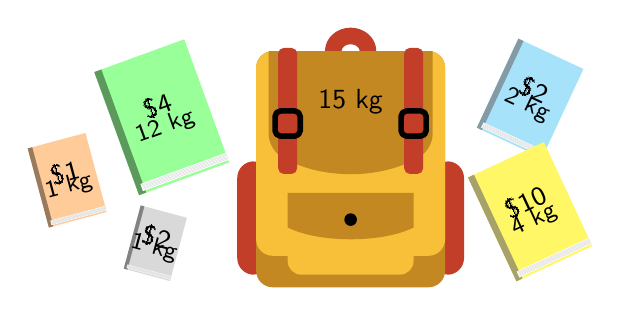
\begin{tikzpicture}[line join=round, line cap=round, font=\sffamily\footnotesize, scale=0.4]

% ---------- helpers ----------
\definecolor{bagyellow}{RGB}{248,188,46}
\definecolor{baggold}{RGB}{230,160,40}
\definecolor{bagred}{RGB}{194,62,40}

% book(pic): (x,y), angle, fill, price, weight, scale
\newcommand{\book}[7]{%
    \colorlet{bookbase}{#4}
    \colorlet{bookback}{bookbase!60!black}
    \colorlet{bookspine}{bookbase!50!white}
  \begin{scope}[shift={(#1,#2)},rotate=#3,scale=#7,]
    % cover
    \fill[rounded corners=0pt,fill=bookbase] (-1.9,-2.6) rectangle (1.9,2.6);
    \fill[rounded corners=0pt,fill=bookback] (-1.9,-2.6) rectangle (-1.6,2.6);
    % pages strip
    \fill[rounded corners=0pt,white] (-1.7,-2.5) rectangle (1.9,-2.2);
    % \draw[black!12, very thin] (-1.65,-2.45) -- (-1.65,-2.25);
    \foreach \y in {-2.45, -2.4, -2.35, -2.3, -2.25}{%
      \draw[black!12, very thin] (-1.65,\y) -- (1.9,\y);
    }
    % text
    \node[align=center,scale=1.2, rotate=#3] at (0,0.5) {\$#5};
    \node[align=center,scale=1.1, rotate=#3] at (0,-0.4) {#6 kg};
  \end{scope}%
}

% ---------- backpack ----------
% side pockets
\fill[bagred,rounded corners=6pt] (-3.6,-3) rectangle (-2.6,0.6);
\fill[bagred,rounded corners=6pt] ( 2.6,-3) rectangle ( 3.6,0.6);

% top handle
\draw[line width=6pt,bagred] (0.55,4.1) arc (0:180:0.55 and 0.48);
% \draw[line width=8pt,bagred] (0,4.1) arc (90:270:0.55 and 0.48);


% main body
\fill[baggold!85!black,rounded corners=6pt] (-3.0,-3.4) rectangle (3.0,4.1);
\fill[bagyellow!95!white,rounded corners=6pt] (-3.0,-2.4) rectangle (3.0,4.1);


% front pocket
\fill[bagyellow!95!white] (-2.0,-0.4) -- (2.0, -0.4) [rounded corners=5pt] -- (2.0,-3) [rounded corners=5pt] -- (-2, -3) [rounded corners=0pt] -- cycle;
\fill[baggold!85!black] (-2.0,-0.4) -- (2.0, -0.4)  -- (2.0,-1.5)  .. controls (1,-2) and (-1,-2) .. (-2, -1.5) -- cycle;
\fill[black] (0,-1.25) circle (0.2);

% flap
\fill[baggold!85!black] (-2.6,4.1) -- (2.6, 4.1) [rounded corners=5pt] -- (2.6, 1) .. controls (1.0, 0) and (-1, 0) .. (-2.6, 1) [rounded corners=0pt] -- cycle;


% shoulder straps + buckles
\fill[rounded corners=2pt,bagred] (-2.3,4.2) rectangle (-1.7,0.2);
\fill[rounded corners=2pt,bagred] ( 2.3,4.2) rectangle ( 1.7,0.2);
\draw[black,rounded corners=2pt, line width=2pt] (-2.4,1.4) rectangle (-1.6,2.2);
\draw[black,rounded corners=2pt, line width=2pt] ( 1.6,1.4) rectangle (2.4,2.2);

% weight label
\node[font=\sffamily] at (0,2.5) {15 kg};

% ---------- books ----------
\book{-6}{2.0}{20}{green!40}{4}{12}{0.8}
\book{-6.2}{-2.0}{-15}{gray!30}{2}{1}{0.4}
\book{-9}{0}{15}{orange!40}{1}{1}{0.5}
\book{5.7}{2.6}{-25}{cyan!35}{2}{2}{0.6}
\book{5.7}{-1.0}{25}{yellow!60}{10}{4}{0.7}

\end{tikzpicture}
\]


% \[
% \operatorname{opt}(i, w) 
% =
% \begin{cases}
% 0 & \text{if } i = 0\\
% \operatorname{opt}(i-1, w) & \text{if } w_i > w\\
% \max\{ v_i + \operatorname{opt}(i-1, w - w_i), \operatorname{opt}(i-1, w)\} & \text{otherwise}
% \end{cases}
% \]
% % where \(i\) is the index of the current item, \(w\) is the remaining weight capacity, \(w_i\) is the weight of item \(i\) and \(v_i\) is the value of item \(i\).     



\definecolor{knapblue}{RGB}{0,130,130}
\definecolor{knapred}{RGB}{180,0,0}
recursive formulation:
\[
\operatorname{opt}(i, w)
=
\left\{
\begin{array}{@{}l@{\quad}l@{\quad}l@{}}
{0}
  & {i = 0}
  & \textcolor{knapred}{\triangleright\ \text{no items left}}\\[0.3em]
{\operatorname{opt}(i-1, w)}
  & {w_i > w}
  & \textcolor{knapred}{\triangleright\ \text{item too heavy}}\\[0.3em]
{\max\{v_i + \operatorname{opt}(i-1, w - w_i),\ \operatorname{opt}(i-1, w)\}}
  & {\text{otherwise}}
  & \textcolor{knapred}{\triangleright\ \text{include or exclude item $i$?}}
\end{array}
\right.
\]



% \begin{algorithmic}[1]
% \Function{opt}{$i, w$}
%   \If{$i = 0$} \Comment{no items left}
%     \State \Return \(0\)
%   \ElsIf{$w_i > w$} \Comment{item too heavy}
%     \State \Return \Call{opt}{$i-1, w$}
%   \Else \Comment{include or exlude item \(i\)?}
%     \State \Return \(\max\{ v_i + \Call{opt}{i-1, w - w_i}, \Call{opt}{i-1, w} \}\)
%   \EndIf
% \EndFunction
% \end{algorithmic}



% \[
% \operatorname{opt}(i,w) 
% =
% \begin{cases}
% 0 & \text{if } i = 0 \text{ (no items left)}\\[0.3em]
% \operatorname{opt}(i-1, w) & \text{if } w_i > w \text{ (too heavy)}\\[0.3em]
% \max\{ v_i + \operatorname{opt}(i-1, w - w_i), \operatorname{opt}(i-1, w)\}
%   & \text{otherwise (include or exclude item $i$?)}
% \end{cases}
% \]



top down memoized:
\begin{algorithm}[h]
\caption{Knapsack (top-down, memoized)}\label{alg:knapsack_topdown}
\begin{algorithmic}[1]
\Function{Opt}{$i, w$}
  \If{\(M[i,w] = \nil\)} 
    \If{\(i = 0\)} 
    \State \(M[i,w] \gets 0\) \Comment{no items left}
    \ElsIf{\(w_i > w\)} 
    \State \(M[i,w] \gets \Call{Opt}{i-1, w}\) \Comment{item too heavy}      
    \Else 
    \State \(M[i,w] \gets \max\{ v_i + \Call{Opt}{i-1, w - w_i}, \Call{Opt}{i-1, w} \}\) \Comment{include or exclude?}
    \EndIf
  \EndIf
  \State \Return \(M[i,w]\)
\EndFunction
\end{algorithmic}
\end{algorithm}


\textcolor{AccentBlue}{Bottom-up (tabulation) version.}
Instead of recursion + memoization, we can fill a DP table iteratively.
Let \(W\) be the knapsack capacity.
We build a table \(\operatorname{OPT}[i,w]\) for \(i = 0,\ldots,n\) and \(w = 0,\ldots,W\),
where
\(
\operatorname{OPT}[i,w]
\)
denotes the maximum value achievable using items \(1,\ldots,i\) with capacity \(w\).


\begin{algorithm}[h]
\caption{Knapsack (bottom-up DP)}\label{alg:knapsack_bottomup}
\begin{algorithmic}[1]
\Require items \(1,\ldots,n\) with weights \(w_i\), values \(v_i\); capacity \(W\)
\For{$w = 0 \TO W$}
  \State \(\operatorname{OPT}[0,w] \gets 0\) \Comment{no items}
\EndFor
\For{$i = 1 \TO n$}
  \For{$w = 0 \TO W$}
    \If{$w_i > w$}
      \State \(\operatorname{OPT}[i,w] \gets \operatorname{OPT}[i-1,w]\) \Comment{item \(i\) too heavy}
    \Else
      \State \(\operatorname{OPT}[i,w] \gets
        \max\bigl\{
          v_i + \operatorname{OPT}[i-1, w - w_i],\;
          \operatorname{OPT}[i-1, w]
        \bigr\}\)
    \EndIf
  \EndFor
\EndFor
\State \Return \(\operatorname{OPT}[n,W]\)
\end{algorithmic}
\end{algorithm}

\textcolor{AccentBlue}{Running time.}
The table has \((n+1)(W+1) = O(nW)\) entries, 
and each is filled in \(O(1)\) time, so the running time is \(O(nW)\) and the space is \(O(nW)\).
By keeping only two rows at a time, the space can be reduced to \(O(W)\).

\begin{remark}
0/1 Knapsack is NP-hard in general, so we do not expect a polynomial-time algorithm in the input size.
The DP runs in time polynomial in \(n\) and \(W\), which is called \emph{pseudo-polynomial} time,
because \(W\) is exponential in the number of bits needed to represent it (i.e. the input size).
\end{remark}









% \clearpage










\subsection{Longest Common Subsequence}
Let us think of character strings as sequences of characters. 
Given $X=\left\langle x_1, \ldots, x_l\right\rangle$, we say that $Z=\left\langle z_1, \ldots, z_k\right\rangle$ is a subsequence of $X$ if there is a strictly increasing sequence of $k$ indices $\left\langle i_1, \ldots, i_k\right\rangle$ such that $Z=\left\langle x_{i_1}, \ldots, x_{i_k}\right\rangle$. 

Given two strings \(X=\left\langle x_1, \ldots, x_m\right\rangle\) and \(Y = \left\langle y_1, \ldots, y_n \right\rangle\), the longest common subsequence of $X$ and $Y$ is a longest sequence $Z$ that is a subsequence of both $X$ and $Y$. 

A prefix \(X_i\) of a sequence \(X\) is just an initial string of values, \(X_i = \langle x_1, \ldots, x_i \rangle\).
\(X_0\) is the empty sequence.
The idea will be to compute the longest common subsequence for every possible pair of prefixes. 
Let $\operatorname{lcs}(i, j)$ denote the length of the longest common subsequence of $X_i$ and $Y_j$.
We have the following recursive relation:
\[
\operatorname{lcs}(i, j)
= 
\begin{cases}
  0 & \text { if } i=0 \text { or } j=0 \\ 
  \operatorname{lcs}(i-1, j-1)+1 & \text { if } i, j>0 \text { and } x_i=y_j \\ 
  \max (\operatorname{lcs}(i-1, j), \operatorname{lcs}(i, j-1)) & \text { if } i, j>0 \text { and } x_i \neq y_j
\end{cases}
\]


Last characters match:
\[
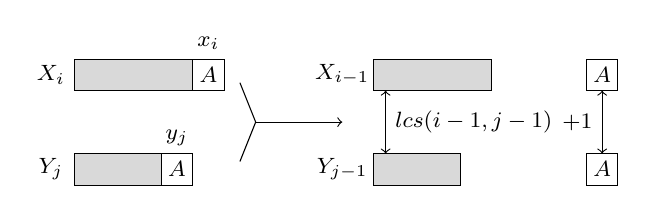
\begin{tikzpicture}[scale=0.5, font=\footnotesize]

%--- left strings Xi, Yj ------------------------------------------
% Xi row
\node at (0,1.2) {$X_i$};
\draw[fill=gray!30] (0.6,0.8) rectangle (3.6,1.6);   % prefix of Xi
\draw              (3.6,0.8) rectangle (4.4,1.6);     % last char
\node at (4.0,1.2) {$A$};
\node at (4.0,2.0) {$x_i$};

% Yj row
\node at (0,-1.2) {$Y_j$};
\draw[fill=gray!30] (0.6,-1.6) rectangle (2.8,-0.8);  % prefix of Yj
\draw              (2.8,-1.6) rectangle (3.6,-0.8);   % last char
\node at (3.2,-1.2) {$A$};
\node at (3.2,-0.4) {$y_j$};

%--- branching + arrow --------------------------------------------
\coordinate (c) at (5.2,0);
\draw (4.8,1.0) -- (c) -- (4.8,-1.0);
\draw[->] (c) -- (7.4,0);

%--- right strings Xi-1, Yj-1 -------------------------------------
% Xi-1 row
\node at (7.4,1.2) {$X_{i-1}$};
\draw[fill=gray!30] (8.2,0.8) rectangle (11.2,1.6);

% Yj-1 row
\node at (7.4,-1.2) {$Y_{j-1}$};
\draw[fill=gray!30] (8.2,-1.6) rectangle (10.4,-0.8);
% vertical lcs arrow and label
\draw[<->] (8.5,0.8) -- (8.5,-0.8);
\node[right] at (8.5,0) {$\operatorname{lcs}(i-1,j-1)$};

%--- "+1" and two A boxes -----------------------------------------
\node[left] at (14,0) {$+1$};

\draw (13.6,0.8)  rectangle (14.4,1.6);
\draw (13.6,-1.6) rectangle (14.4,-0.8);
\node at (14.0,1.2) {$A$};
\node at (14.0,-1.2) {$A$};
\draw[<->] (14.0,0.8) -- (14.0,-0.8);

\end{tikzpicture}
\]


Last characters do not match:
\[
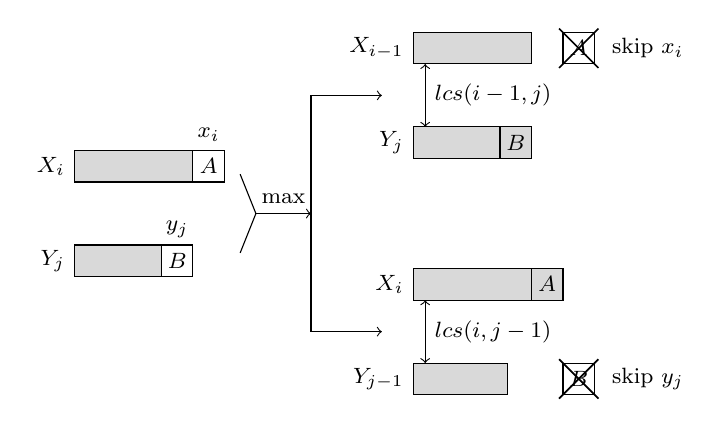
\begin{tikzpicture}[scale=0.5, font=\footnotesize]

%--- left strings Xi, Yj ------------------------------------------
% Xi row
\node[left] at (0.6,1.2) {$X_i$};
\draw[fill=gray!30] (0.6,0.8) rectangle (3.6,1.6);   % prefix of Xi
\draw              (3.6,0.8) rectangle (4.4,1.6);     % last char
\node at (4.0,1.2) {$A$};
\node at (4.0,2.0) {$x_i$};

% Yj row
\node[left] at (0.6,-1.2) {$Y_j$};
\draw[fill=gray!30] (0.6,-1.6) rectangle (2.8,-0.8);  % prefix of Yj
\draw              (2.8,-1.6) rectangle (3.6,-0.8);   % last char
\node at (3.2,-1.2) {$B$};
\node at (3.2,-0.4) {$y_j$};

%--- branching + arrow --------------------------------------------
\coordinate (c) at (5.2,0);
\draw (4.8,1.0) -- (c) -- (4.8,-1.0);
\draw[->] (c) -- (6.6,0);
\node[above] at (5.9,0) {$\max$};
\draw (6.6,3.0) -- (6.6,-3.0);
\draw[->] (6.6,3) -- (8.4,3);
\draw[->] (6.6,-3) -- (8.4,-3);


\begin {scope}[shift={(1, 3)}]
%--- right strings Xi-1, Yj-1 -------------------------------------
% Xi-1 row
\node[left] at (8.2,1.2) {$X_{i-1}$};
\draw[fill=gray!30] (8.2,0.8) rectangle (11.2,1.6);

\draw (12,0.8) rectangle (12.8,1.6);
\node at (12.4,1.2) {$A$};

% cross
\draw[line width=0.6pt] (11.9,0.7) -- (12.9,1.7);
\draw[line width=0.6pt] (11.9,1.7) -- (12.9,0.7);
\node[right] at (13,1.2) {skip $x_i$};

% Yj-1 row
\node[left] at (8.2,-1.2) {$Y_{j}$};
\draw[fill=gray!30] (8.2,-1.6) rectangle (10.4,-0.8);
\draw[fill=gray!30] (10.4,-1.6) rectangle (11.2,-0.8);
\node at (10.8,-1.2) {$B$};
% vertical lcs arrow and label
\draw[<->] (8.5,0.8) -- (8.5,-0.8);
\node[right] at (8.5,0) {$\operatorname{lcs}(i-1,j)$};
\end{scope}

\begin {scope}[shift={(1, -3)}]
%--- right strings Xi-1, Yj-1 -------------------------------------
% Xi-1 row
\node[left] at (8.2,1.2) {$X_{i}$};
\draw[fill=gray!30] (8.2,0.8) rectangle (11.2,1.6);
\draw[fill=gray!30] (11.2,0.8) rectangle (12.0,1.6);
\node at (11.6,1.2) {$A$};

% Yj-1 row
\node[left] at (8.2,-1.2) {$Y_{j-1}$};
\draw[fill=gray!30] (8.2,-1.6) rectangle (10.6,-0.8);

\draw (12.0,-1.6) rectangle (12.8,-0.8);
\node at (12.4,-1.2) {$B$};

% cross
\draw[line width=0.6pt] (11.9,-1.7) -- (12.9,-0.7);
\draw[line width=0.6pt] (11.9,-0.7) -- (12.9,-1.7);
\node[right] at (13, -1.2) {skip $y_j$};


% vertical lcs arrow and label
\draw[<->] (8.5,0.8) -- (8.5,-0.8);
\node[right] at (8.5,0) {$\operatorname{lcs}(i,j-1)$};
\end{scope}


\end{tikzpicture}
\]





\textcolor{AccentBlue}{DP table.}
We store values in a table \(L[0\ldots m, 0\ldots n]\) where
\(L[i,j] = \operatorname{lcs}(i,j)\).

\begin{algorithm}[h]
\caption{Longest Common Subsequence (bottom-up DP)}\label{alg:lcs}
\begin{algorithmic}[1]
\Require strings \(X = x_1\cdots x_m\), \(Y = y_1\cdots y_n\)
\For{$i = 0 \TO m$}
  \State \(L[i,0] \gets 0\)
\EndFor
\For{$j = 0 \TO n$}
  \State \(L[0,j] \gets 0\)
\EndFor
\For{$i = 1 \TO m$}
  \For{$j = 1 \TO n$}
    \If{$x_i = y_j$}
      \State \(L[i,j] \gets L[i-1,j-1] + 1\)
    \Else
      \State \(L[i,j] \gets \max\{L[i-1,j], L[i,j-1]\}\)
    \EndIf
  \EndFor
\EndFor
\State \Return \(L[m,n]\)
\end{algorithmic}
\end{algorithm}

To reconstruct an actual LCS (not just its length), we can backtrack from \((m,n)\) towards \((0,0)\):
If \(x_i = y_j\) and \(L[i,j] = L[i-1,j-1]+1\), then \(x_i\) is part of some LCS and we move to \((i-1,j-1)\); 
otherwise, if \(L[i-1,j] \ge L[i,j-1]\) move to \((i-1,j)\), else move to \((i,j-1)\).

\textcolor{AccentBlue}{Running time.}
The table has \((m+1)(n+1) = O(mn)\) entries, each filled in \(O(1)\) time,
so the running time is \(O(mn)\) and the space is \(O(mn)\) (or \(O(\min\{m,n\})\) if we only need the length).









\subsection{Shortest Paths with Negative Weights}

% \nameref{alg:bellmanford} algorithm is a dynamic-programming, label-correcting method that supports arbitrary (i.e. including negative) weights and detects negative-weight cycles.  
% It relaxes all edges in up to \( n-1\) passes for \(O( n\times m)\) time and uses one extra pass to check for cycles.

% The Bellman-Ford equation:
% \begin{equation}\label{eq:bellmanford}
% \delta(s, v) = \min_{(u,v)\in E} \left(\delta(s, u) + w(u, v)\right)
% \end{equation}

% \begin{algorithm}[h]
% \caption{Bellman-Ford}\label{alg:bellmanford}
% \begin{algorithmic}[1]
% \Function{BellmanFord}{$G, w:E\to\R, s$}
%   \ForAll{$v\in V(G)$}
%     \State $\attrib{v}{\delta}\gets\infty$
%     \State $\attrib{v}{\pi}\gets\nil$
%   \EndFor
%   \State $\attrib{s}{\delta}\gets 0$
%   \For{$i=1$ to $|V(G)|-1$} 
%     \ForAll{$(u,v)\in E(G)$}
%       \If{$\attrib{u}{\delta}+w(u,v)<\attrib{v}{\delta}$} 
%         \State $\attrib{v}{\delta}\gets \attrib{u}{\delta}+w(u,v)$ \Comment{applying Equation~\eqref{eq:bellmanford}}
%         \State $\attrib{v}{\pi}\gets u$
%       \EndIf
%     \EndFor
%   \EndFor
%   \ForAll{$(u,v)\in E(G)$}
%     \If{$\attrib{u}{\delta}+w(u,v)<\attrib{v}{\delta}$}
%       \State \Return \fals \Comment{negative-weight cycle detected}
%     \EndIf
%   \EndFor
%   \State \Return \tru
% \EndFunction
% \end{algorithmic}
% \end{algorithm}



For graphs with possibly negative edge weights (but no negative-weight cycles reachable from the source),
\nameref{alg:dijkstra}'s greedy algorithm no longer works.
The \nameref{alg:bellmanford} algorithm is a dynamic-programming, label-correcting method that works for arbitrary real edge weights and detects negative-weight cycles.


\textcolor{AccentBlue}{DP viewpoint.}
Let \(G = (V,E)\) be a directed graph with edge weights \(w:E\to\R\), and let \(s\) be the source.
Define
\(
\operatorname{OPT}(i,v)
\)
to be the \hl{length of the shortest \(s\)-\(v\) path that uses \emph{at most} \(i\) edges}.
\begin{itemize}
  \item Base cases (\(i=0\)):
  \(
  \operatorname{OPT}(0,s) = 0
  \), 
  \(
  \operatorname{OPT}(0,v) = \infty
  \) for \(v \neq s\)
  \item For \(i \ge 1\) and any \(v \in V\),
  \[
  \operatorname{OPT}(i,v)
  =
  \min\Bigl\{
    \operatorname{OPT}(i-1,v),\;
    \min_{(u,v)\in E}\bigl(\operatorname{OPT}(i-1,u) + w(u,v)\bigr)
  \Bigr\}
  \]
\end{itemize}

\hl[2]{Any simple path in a graph on \(n\) vertices has at most \(n - 1\) edges}.
If there is no negative-weight cycle reachable from \(s\), the shortest paths are simple,
so the true shortest-path distances are given by \(\operatorname{OPT}(n-1,v)\).


Instead of explicitly storing the 2D table \(\operatorname{OPT}(i,v)\),
Bellman-Ford iteratively relaxes all edges in the graph.

\begin{algorithm}[h]
\caption{Bellman-Ford}\label{alg:bellmanford}
\begin{algorithmic}[1]
\Function{BellmanFord}{$G,w:E\to\R,s$}
  \ForAll{$v \in V(G)$}
    \State \(\attrib{v}{\delta} \gets \infty\)
    \State \(\attrib{v}{\pi} \gets \nil\) \Comment{predecessor on shortest path tree}
  \EndFor
  \State \(\attrib{s}{\delta} \gets 0\)
  \For{$i = 1 \TO |V(G)| - 1$} \Comment{at most \(|V|-1\) edges on a simple path}
    \ForAll{$(u,v) \in E(G)$}
      \If{\(\attrib{u}{\delta} + w(u,v) < \attrib{v}{\delta}\)}
        \State \(\attrib{v}{\delta} \gets \attrib{u}{\delta} + w(u,v)\)
        \State \(\attrib{v}{\pi} \gets u\)
      \EndIf
    \EndFor
  \EndFor
  \ForAll{$(u,v) \in E(G)$}
    \If{\(\attrib{u}{\delta} + w(u,v) < \attrib{v}{\delta}\)}
      \State \Return \fals \Comment{negative-weight cycle detected}
    \EndIf
  \EndFor
  \State \Return \tru \Comment{distances \(\attrib{v}{\delta}\) are correct}
\EndFunction
\end{algorithmic}
\end{algorithm}

\textcolor{AccentBlue}{Running time.}
The algorithm performs \(O(|V|)\) passes, each relaxing all \(|E|\) edges once.
Thus the running time is \(O(|V|\cdot|E|)\) and the space usage is \(O(|V|)\).
The \(\attribute{\pi}\) pointers define a shortest-path tree rooted at \(s\).



